% Metódy inžinierskej práce

%Toto je fess super dobrý článok! :0

\documentclass[10pt,twoside,slovak,a4paper]{article}

\usepackage[slovak]{babel}
%\usepackage[T1]{fontenc}
\usepackage[IL2]{fontenc} % lepšia sadzba písmena Ľ než v T1
\usepackage[utf8]{inputenc}
\usepackage{graphicx}
\usepackage{url} % príkaz \url na formátovanie URL
\usepackage{hyperref} % odkazy v texte budú aktívne (pri niektorých triedach dokumentov spôsobuje posun textu)

\usepackage{cite}
%\usepackage{times}

\pagestyle{headings}

\title{Pomoc deťom s ASD s výrazmi tváre pomocou hier\thanks{Semestrálny projekt v predmete Metódy inžinierskej práce, ak. rok 2022/23, vedenie: Ing. Mohammed Yusuf Momand, MSc.}} % meno a priezvisko vyučujúceho na cvičeniach

\author{Martin Matloha\\[2pt]
	{\small Slovenská technická univerzita v Bratislave}\\
	{\small Fakulta informatiky a informačných technológií}\\
	{\small \texttt{xmatloha@stuba.sk}}
	}

\date{\small 6. november 2022} % upravte



\begin{document}

\maketitle

\begin{abstract}
V mojom článku by som sa chcel zamerať na hry, ktoré pomáhajú deťom s poruchou autistického spektra (ASD). Deti s touto poruchou si často nerozumejú s inými deťmi kvôli ich inému sociálnemu správaniu a pohľadom na svet. To môže viesť k úzkosti až depresii u takýchto detí. Výskum sa zameriava na rozpoznávanie alebo produkciu emócií a rozvoj sociálnych zručností u detí s ASD/Aspergerom. Hry s takýmto zameraním sú pre deti lákavejšie ako iné metódy liečby a s neustálym pokrokom v oblasti hier môže byť takáto liečba aj účinnejšia. V článku sa zaoberám jedným z takýchto problémov, ktorým je ťažšia produkcia a detekcia emócií pomocou tváre u takýchto detí.
\end{abstract}



\section{Úvod}
Zo všeobecného pohľadu človeka sa ľudská tvár skladá z rovnakých čŕt, teda bežný človek má na tvári dve oči, nos, ústa.  Samozrejme, každá tvár je mierne odlišná, čo sa týka závislosti jednej črty od druhej. Vďaka tomu sa vieme navzájom rozpoznávať s určitou ľahkosťou, ale iba v prípade, že máme schopnosť vnímať tvár ako celok. Pričom niektorí ľudia túto schopnosť nemajú. Tento problém je podrobnejšie vysvetlený v časti~\ref{problematika}.

Očákavaný výsledok pri riešení problému a prekážky v tejto problematike sú uvedené v častiach~\ref{ocakavanie} a~\ref{prekazky}.

Záverečné poznámky prináša časť~\ref{zaver}.



\section{Stav riešenia problematiky} \label{stav}

Na základe počtu nájdených článkov v databáze SCOPUS podľa vyhľadávania kľúčových slov \emph{``emotions AND asd AND autism AND ''facial recognition''``} som sa rozhodol posúdiť, ako veľmi sa verejnosť venuje tejto problematike. Na obr.~\ref{f:rozhod} môžete vidieť graf utvorený z vyššie spomenutého vyhľadávania. Zistil som, že pred rokom 2016 bola táto problematika relatívne zanedbávaná. Našťastie, posledné roky pozorujeme nárast počtu článkov až do 28 článkov za rok, z čoho by som vyvodil, že sa táto problematika rozoberá viac.

\begin{figure*}[tbh]
\centering
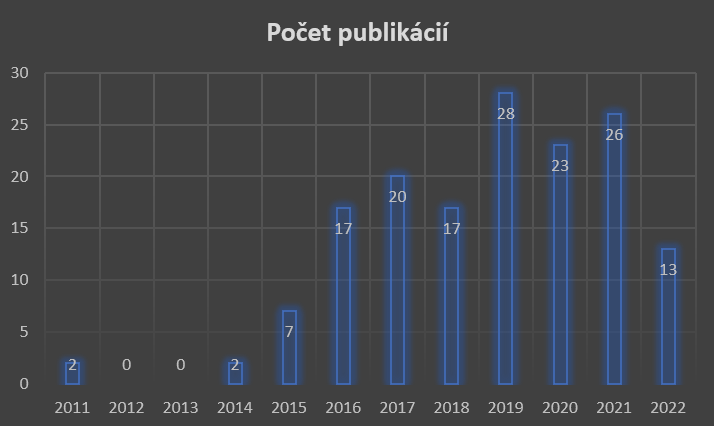
\includegraphics[scale=1]{graf.png}
%Aj text môže byť prezentovaný ako obrázok. Stane sa z neho označný plávajúci objekt. Po vytvorení diagramu zrušte znak \texttt{\%} pred príkazom \verb|\includegraphics| označte tento riadok ako komentár (tiež pomocou znaku \texttt{\%}).
\caption{Počet publikácií.}
\label{f:rozhod}
\end{figure*}



\section{Problematika} \label{problematika}
Základným problémom je teda ťažkosť detí s ASD od seba odlišovať ľudské tváre a rozlišovať emócie a s nimi spojené výrazy tváre. Tento problém vedie ku zníženému pochopeniu sociálnych situácií vedúcim ku horšiemu kontaktu s ľuďmi.   

Zdá sa, že problém spôsobuje odlišné vnímanie a spracuvávanie tvárí. Narozdiel od bežného človeka, ktorý sa na tvár pozerá ako na celok, sa ľudia s ASD zameriavajú skôr na jednotlivé časti tváre (oči, uši, ústa, nos,\ldots{})~\cite{Avatar-Assistant}.

Obtiažnosť identifikácie pocitov sa líši podľa zamerania sa na konkrétnu časť tváre. Pričom pri zameraní sa na oblasť úst vedeli deti s ASD ľahšie identifikovať prejavenú emóciu ako pri zameraní na oči.\ldots{})~\cite{Avatar-Assistant}. 

Vyvinutie schopností rozpoznania tvárí, emócií a výrazov v každodennom živote je pre dieťa dôležitým krokom ku zaradeniu sa do spoločnosti. Vedie to ku tvorbe nových doživotných priateľstiev a kontaktov, čo uľahčuje priebeh života. 

\underline{\emph{ Základné pocity:}}
\begin{itemize}
\item Šťastie
\item Smútok
\item Hnev
\item Prekvapenie
\item Strach
\item Znechutenie	
\end{itemize}


%Základným problémom je teda\ldots{} Najprv sa pozrieme na nejaké vysvetlenie (časť~\ref{ina:nejake}), a potom na ešte nejaké (časť~\ref{ina:nejake}).\footnote{Niekedy môžete potrebovať aj poznámku pod čiarou.}

%Môže sa zdať, že problém vlastne nejestvuje\cite{Coplien:MPD}, ale bolo dokázané, že to tak nie je~\cite{Czarnecki:Staged, Czarnecki:Progress}. Napriek tomu, aj dnes na webe narazíme na všelijaké pochybné názory\cite{PLP-Framework}. Dôležité veci možno \emph{zdôrazniť kurzívou}.


\subsection{Metódy riešenia} \label{problematika:metody}

Podľa kontaktu:

\begin{itemize}
\item S ľudským kontaktom
\item Bez ľudského kontaktu
	\begin{itemize}
	\item Digitálne
	\item Analógovo
	\end{itemize}
\end{itemize}



%\begin{enumerate}
%\item jedna vec
%\item druhá vec
%	\begin{enumerate}
%	\item x
%	\item y
%	\end{enumerate}
%\end{enumerate}


\subsection{Riešenie pomocou hier} \label{problematika:hry}

\paragraph{Veľmi dôležitá poznámka.}
Niekedy je potrebné nadpisom označiť odsek. Text pokračuje hneď za nadpisom.



\section{Očakávaný výsledok} \label{ocakavanie}




\section{Prekážky pri riešení problému} \label{prekazky}




\section{Záver} \label{zaver} % prípadne iný variant názvu



%\acknowledgement{Ak niekomu chcete poďakovať\ldots}


% týmto sa generuje zoznam literatúry z obsahu súboru literatura.bib podľa toho, na čo sa v článku odkazujete
\bibliography{literatura}
\bibliographystyle{plain} % prípadne alpha, abbrv alebo hociktorý iný
\end{document}
